\documentclass[conference,a4paper]{IEEEtran}
\IEEEoverridecommandlockouts
\usepackage[T1]{fontenc}
\usepackage{cite}
\usepackage{amsmath,amssymb,amsfonts}
\usepackage{graphicx}
\usepackage{textcomp}
\usepackage{booktabs}
\usepackage{multirow}
\usepackage[hyphens]{url}
\usepackage{tikz}
\usetikzlibrary{arrows.meta,positioning}

\newcommand{\pol}[1]{\texttt{\detokenize{#1}}}

\begin{document}

\title{Adaptive Zero-Shot Document Extraction with Safe Policy Routing: Design and Paired Evaluation of a Local OCR--LLM Pipeline}

% Double-blind submission: replace with the author block only for camera-ready or single-blind venues.
\author{\IEEEauthorblockN{Omitted for blind review}}

\maketitle

\begin{abstract}
Template-free document extraction with local OCR and a large language model (LLM) removes most setup cost, but one fixed configuration rarely suits every document. We ask whether an online bandit router that selects among declarative processing policies per document improves zero-shot extraction, and how such a router can be deployed safely. Our system runs PaddleOCR and a 9.7B-parameter LLM locally. A router (AHMN) applies Bernoulli Thompson sampling over the eligible policies, and an \emph{adaptive\_safe} gate falls back when a candidate regresses relative to the default policy. We compare this configuration with a static default-only baseline in paired runs over 133 documents in four packs (126 unique): 100 CORD~v2 receipts split into a development pack and a disjoint holdout, 20 FUNSD forms, and 13 hard documents with skew, fading, fax noise and multiple pages. Adaptive routing did not improve accuracy. On the 100 receipts, mean document F1 changed by $-0.011$ (95\% CI $[-0.038, 0.011]$) while latency rose by 3.9~s per document, and every FUNSD and hard document was tied. We trace this to a label-free reward that credits filling fields rather than filling them correctly, and to an action space in which only two policies change the extraction call. We also show that absolute latency limits silently disabled adaptation in our first runs, and that a baseline-relative guard restored exploration without loss of accuracy. We release the pipeline, the benchmark packs and the evaluation scripts, and report simulation-only results for two extensions aimed at cold start and drift.
\end{abstract}

\begin{IEEEkeywords}
document AI, intelligent document processing, zero-shot information extraction, large language models, Thompson sampling, safe exploration, OCR
\end{IEEEkeywords}

\section{Introduction}
\label{sec:intro}

Organisations process invoices, receipts, forms and letters that vary in layout, scan quality and terminology. Commercial intelligent document processing (IDP) platforms reach high accuracy once configured, but configuration is the cost: document definitions and field regions~\cite{abbyyfields}, taxonomies of document types and fields~\cite{uipath}, labelled data for custom models~\cite{azurecustom}, or adapters trained on annotated samples~\cite{textractcustom}. Local OCR combined with an instruction-following LLM offers a different operating point: the user names the fields, and the system extracts them from unseen layouts without templates, training or a cloud service.

Such pipelines expose many choices, including image preprocessing, OCR settings, whether to request all fields in one call or one field at a time, what context to give the model, and how to recover failed fields. No single setting is best for every document, which suggests learning the choice online. Multi-armed bandits are the standard tool for this~\cite{lattimore2020}, and Thompson sampling~\cite{thompson1933,chapelle2011} is simple and effective. Two practical obstacles remain. Ground-truth labels are not available at run time, so the router must learn from a proxy reward. And an exploring router can send production documents to a worse policy, so exploration must be bounded.

We built a system to study these questions. Its orchestrator (IDPO) turns each document into a policy-conditioned execution plan, its router (AHMN) recommends the policy, and a safety gate decides whether the recommendation is used. We compare this adaptive configuration with a static baseline that always uses the default policy, in paired runs that include a held-out split.

The contributions are:
\begin{enumerate}
\item A locally deployable, template-free extraction pipeline in which a declarative policy governs each document's processing and every run writes auditable per-document artifacts (Section~\ref{sec:system}).
\item An \emph{adaptive\_safe} routing layer: Bernoulli Thompson sampling over condition-eligible policies, and a rollback monitor whose limits are set relative to the default policy's recent behaviour (Section~\ref{sec:routing}).
\item A paired evaluation on four benchmark packs with a development/holdout split, per-document bootstrap intervals, and a disclosure of which policy fields actually change runtime behaviour (Sections~\ref{sec:setup} and~\ref{sec:results}).
\item Two negative findings with practical value: adaptive routing matched but did not beat the static baseline and cost latency on receipts, and absolute guard limits silently turned the adaptive system into a static one (Section~\ref{sec:results}).
\end{enumerate}
We also implemented retrieval-augmented bandit initialisation (RABI) and drift-aware adaptive forgetting (DAAF) for cold start and drift. Neither is active in the measured runtime, and we report both as simulation results only (Section~\ref{sec:simulation}).

\section{Related Work}

\subsection{Configured and Trained Document Understanding}
Research models learn text and layout jointly (LayoutLM~\cite{layoutlm}, LayoutLMv2~\cite{layoutlmv2}, LayoutLMv3~\cite{layoutlmv3}) or read pixels directly (Donut~\cite{donut}, Pix2Struct~\cite{pix2struct}), and question answering benchmarks such as DocVQA~\cite{docvqa} broadened the task. These approaches reach high accuracy on CORD~\cite{cord} and FUNSD~\cite{funsd} after supervised fine-tuning, and commercial platforms need the configuration described in Section~\ref{sec:intro}. Our setting uses no fine-tuning, templates or demonstrations. We use PaddleOCR~\cite{ppocr} for text recognition.

\subsection{LLM-Based Extraction}
Instruction-tuned LLMs can extract fields from OCR text given only field names and short descriptions. ICL-D3IE~\cite{icld3ie} selects in-context demonstrations for document information extraction, and LLM-driven methods have been applied to non-standard tables~\cite{llmtkie}. Our extractor is zero-shot and uses no demonstrations; this paper studies the routing layer around it.

\subsection{Bandits, Drift and Safe Exploration}
Thompson sampling selects actions by sampling from posterior beliefs~\cite{thompson1933,chapelle2011}. Non-stationary bandits~\cite{besbes2014} and the concept-drift literature~\cite{gama2014} address changing reward distributions. Conservative bandits~\cite{wu2016conservative} constrain exploration so that cumulative reward stays above a fraction of a baseline policy's reward. Our gate applies a simpler, operational form of this idea: compare each candidate with the baseline's recent outcomes in the same job, and fall back when the candidate regresses. RABI draws on retrieval augmentation~\cite{rag} and sentence embeddings~\cite{sbert}.

\section{System}
\label{sec:system}

\begin{figure}[t]
\centering
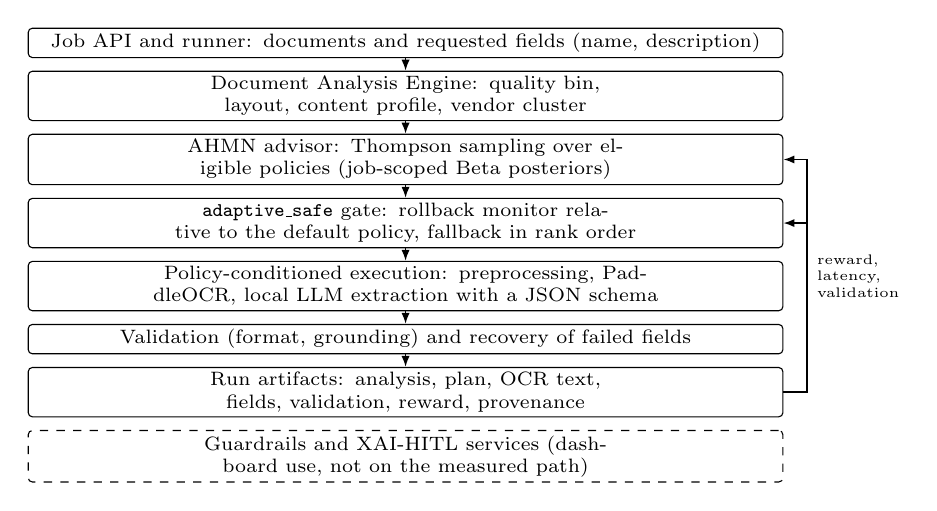
\begin{tikzpicture}[
  node distance=1.6mm,
  box/.style={draw, rounded corners=1.5pt, align=center, font=\scriptsize, text width=0.78\columnwidth, inner sep=1.8pt},
  ext/.style={box, dashed},
  arr/.style={-{Latex[length=1.4mm]}, semithick},
]
\node[box] (job) {Job API and runner: documents and requested fields (name, description)};
\node[box, below=of job] (dae) {Document Analysis Engine: quality bin, layout, content profile, vendor cluster};
\node[box, below=of dae] (ahmn) {AHMN advisor: Thompson sampling over eligible policies (job-scoped Beta posteriors)};
\node[box, below=of ahmn] (gate) {\texttt{adaptive\_safe} gate: rollback monitor relative to the default policy, fallback in rank order};
\node[box, below=of gate] (exec) {Policy-conditioned execution: preprocessing, PaddleOCR, local LLM extraction with a JSON schema};
\node[box, below=of exec] (val) {Validation (format, grounding) and recovery of failed fields};
\node[box, below=of val] (art) {Run artifacts: analysis, plan, OCR text, fields, validation, reward, provenance};
\node[ext, below=of art] (svc) {Guardrails and XAI-HITL services (dashboard use, not on the measured path)};
\foreach \a/\b in {job/dae, dae/ahmn, ahmn/gate, gate/exec, exec/val, val/art} \draw[arr] (\a) -- (\b);
\draw[arr] (art.east) -- ++(3mm,0) coordinate (fb) |- node[pos=0.25, right, font=\tiny, align=left] {reward,\\latency,\\validation} (ahmn.east);
\draw[arr] (fb |- gate.east) -- (gate.east);
\end{tikzpicture}
\caption{Measured runtime path. The reward updates the job's posteriors; latency, validation and reward outcomes feed the rollback monitor. Guardrails and XAI-HITL are separate services, not called by the evaluated pipeline.}
\label{fig:arch}
\end{figure}

\subsection{Runtime Path}
A user creates a job, uploads documents and defines the fields to extract, each with a name and a short description. Starting a run invokes the IDPO pipeline on the selected files (Fig.~\ref{fig:arch}). Every document produces a directory of artifacts: document analysis, routing decision, execution plan, OCR text, extracted fields, validation report, recovery trace, reward and provenance. The Guardrails service (schema, PII and consistency checks) and the XAI-HITL service (explanations and human review) are used from the dashboard but not on the measured path, so no result below depends on them.

\subsection{Document Analysis}
Before OCR, the Document Analysis Engine (DAE) computes a quality bin from image statistics, a structural document type, a content profile and a vendor cluster. In our benchmarks the vendor cluster is the case-identifier prefix of the file name (for example \pol{cord_} or \pol{funsd_}). A semantic document type (receipt, correspondence, form) is defined on OCR text. Because routing happens before OCR, it was \pol{unknown} for every document in our runs (Section~\ref{sec:threats}).

\subsection{Extraction, Validation and Recovery}
Images are upscaled to at least 1600~px, converted to greyscale, contrast-stretched and sharpened. They are deskewed and denoised when the policy or the quality heuristic asks for it, and then read by PaddleOCR~\cite{ppocr}. Extraction calls Qwen3.5 (9.7B parameters, Q4\_K\_M quantisation) through Ollama with temperature~0, top-$p$~0.8, top-$k$~20, an 8192-token context and the reasoning mode disabled. A JSON schema restricts the output to the requested field names, and the prompt asks the model to omit absent fields rather than guess. Validation checks value formats and a grounding rule: every token longer than three characters in an extracted value must occur in the OCR text, and values that fail are flagged. The recovery stage re-extracts failed fields once.

\subsection{Policies}
A policy is a JSON record with eligibility conditions and an actions block covering preprocessing, OCR, extraction, execution mode, recovery and escalation. The research store has 16 policies: a receipt specialist, a correspondence specialist, 13 generic policies oriented to quality, layout or speed, and \pol{default}. Conditions on identity keys (vendor cluster, semantic document type) are combined with OR and all other conditions with AND.

Table~\ref{tab:actions} lists what the actions change in the measured configuration. Several declared settings are recorded in the plan but do not alter the output under PaddleOCR with job-defined fields: Tesseract page-segmentation modes and passes, which apply only if Tesseract runs; the recovery strategy; retrieval and token budgets; and chunking. The two specialists differ from \pol{default} in ways that do matter: they make one LLM call per requested field instead of one call for all fields, and they add a document-type context paragraph to the prompt. The effective action space therefore contains four behaviours, not sixteen, which bounds what any router can gain.

\begin{table}[t]
\caption{What each policy changes in the measured configuration}
\label{tab:actions}
\centering
\footnotesize
\setlength{\tabcolsep}{4pt}
\begin{tabular}{@{}lp{0.48\columnwidth}@{}}
\toprule
Policy & Effect relative to \pol{default}\\
\midrule
\pol{default} & Quality-gated deskew and denoise, one call for all fields, all stages\\
\pol{receipt_specialist} & Per-field extraction, receipt context, extraction-only stages\\
\pol{correspondence_specialist} & Per-field extraction, correspondence context, extraction-only stages\\
\pol{fast_local_text} & Deskew and denoise off\\
5 generic policies & Extraction-only stages (latency only)\\
7 generic policies & No effect on extracted values\\
\bottomrule
\end{tabular}
\end{table}

\section{Adaptive Routing}
\label{sec:routing}

\subsection{Thompson Sampling over Eligible Policies}
For each job, AHMN keeps a Beta posterior $\theta_p \sim \mathrm{Beta}(\alpha_p, \beta_p)$ per policy~$p$. For a document, the candidate set contains the policies whose conditions match plus \pol{default}. If a specialist is eligible, the quality-oriented generic policies are removed from the draw (specialist exclusivity). AHMN draws $\theta_p$ for every candidate and recommends the policy with the largest draw. Specialists start from $\mathrm{Beta}(3,1)$. If the job's mean field success rate $\bar s$ is below 0.5 when a specialist's posterior is created, its $\alpha$ starts at $3 + 2\min(1, 2(0.5-\bar s))$ instead, at most~5. \pol{default} and six receipt- and quality-oriented generic policies start from $\mathrm{Beta}(1.5,1)$, and the rest from $\mathrm{Beta}(1,1)$. After the document is processed, the chosen policy receives a Bernoulli update from the reward $r\in[0,1]$:
\begin{equation}
\alpha_p \leftarrow \alpha_p + \mathbb{1}[r \ge \tfrac{1}{2}], \qquad \beta_p \leftarrow \beta_p + \mathbb{1}[r < \tfrac{1}{2}].
\end{equation}
Posteriors are scoped to a job, so every new job starts from the priors.

\subsection{Label-Free Reward}
Labels are not available at run time. Let $Q$ be the requested fields and $E$ the fields that received a concrete value. With $\mathrm{TP}=|E\cap Q|$, $\mathrm{FN}=|Q\setminus E|$ and $\mathrm{FP}=|E\setminus Q|$, the reward is
\begin{equation}
r = \frac{2\,\mathrm{TP}}{2\,\mathrm{TP}+\mathrm{FP}+\mathrm{FN}}.
\end{equation}
This measures coverage, not correctness. A policy that fills every requested field with a wrong value earns $r=1$, and a policy that correctly leaves out a field missing from the document is penalised. Because the JSON schema restricts outputs to the requested names, FP is almost always zero, and $r$ reduces to the fraction of requested fields that were filled.

\subsection{The adaptive\_safe Gate}
The gate receives the advisor's recommendation followed by a rule-based ranking of all policies by how well their conditions match the document. It takes the first policy in this list whose conditions match and that the rollback monitor does not block, and uses \pol{default} if none qualifies. For each non-default policy~$p$, the monitor keeps the last $W=10$ outcomes in the job: latency, validation pass or fail, and reward. Once $p$ has at least $m=\min(5,W)$ outcomes, it is blocked if
\begin{equation}
\begin{gathered}
\mathrm{p95}(\ell_p) > L_p, \quad f_p > F_p, \quad \text{or} \quad \bar r_{d} - \bar r_p > \delta_q, \\
L_p = \max\!\big(L, (1+\rho)\,\mathrm{p95}(\ell_d)\big), \qquad F_p = \max\!\big(F, f_d + \delta_v\big),
\end{gathered}
\end{equation}
where $\ell$, $f$ and $\bar r$ are latency, validation failure rate and mean reward, and $d$ is \pol{default}. The relative terms apply once the default has at least $m$ outcomes; before that, the absolute limits $L$ and $F$ apply alone. We use $L=60$~s, $F=0.5$, $\rho=0.25$, $\delta_v=0.10$ and $\delta_q=0.08$. Our first runs used absolute limits only (Section~\ref{sec:guard}).

\section{Experimental Setup}
\label{sec:setup}

\subsection{Conditions}
The \emph{static} condition uses a policy store that contains only \pol{default}, with the router disabled. The \emph{adaptive\_safe} condition uses the 16-policy research store, the router and the gate. Everything else is shared: images, OCR, LLM, prompts, validation, recovery and scorer. Each document is processed once per condition, with up to four documents in parallel.

\subsection{Benchmark Packs}
Table~\ref{tab:packs} lists the packs. CORD-dev is a seed-17 sample of 50 receipts from the CORD~v2 validation split~\cite{cord}. We used it while developing prompts, normalisers and the receipt specialist's context. CORD-holdout contains the other 50 validation receipts and was not used during development. All CORD packs use the five summary fields that CORD annotates: total, subtotal, tax, cash and change. FUNSD-20 contains test-split forms~\cite{funsd} with linked question--answer annotations for date, recipient and sender. HARD-13 is a stress pack. It contains six synthetic documents with known ground truth (a skewed image-only invoice, a faded receipt photograph, a letter photograph, a fax-quality claim form, a two-page scanned purchase order and a dense digital bank statement), four CORD receipts and three FUNSD forms. Those seven real documents also appear in the other packs, so the four packs contain 133 document instances and 126 unique documents. For the CORD and FUNSD packs, each condition processes the whole pack as one job, so posteriors and the rollback window accumulate over up to 50 documents. HARD-13 runs one job per document, so each starts from the priors; it tests cold-start routing and the gate, not learning.

\begin{table}[t]
\caption{Benchmark packs}
\label{tab:packs}
\centering
\footnotesize
\setlength{\tabcolsep}{3pt}
\begin{tabular}{lccll}
\toprule
Pack & Docs & Labels & Fields & One job per\\
\midrule
CORD-dev & 50 & 160 & 5 receipt totals & condition\\
CORD-holdout & 50 & 180 & 5 receipt totals & condition\\
FUNSD-20 & 20 & 47 & date, recipient, sender & condition\\
HARD-13 & 13 & 51 & 4--6 per document & document\\
\bottomrule
\end{tabular}
\end{table}

\subsection{Scoring}
Numeric fields are compared exactly after normalisation: the currency prefix, spaces and commas are removed, dots that separate groups of exactly three digits are read as thousands separators, and trailing decimal zeros are removed. Text fields are lowercased and normalised, which unifies date separators, corrects common OCR misspellings of month names and removes dots in initials. They match if the normalised strings are equal or their sequence-matcher similarity is at least 0.75. Date fields also match when both strings name the same complete calendar date; partial dates never match a full one. A wrong value counts as one false positive and one false negative, a missing value as one false negative, and a value for an unlabelled field as one false positive. We report micro precision, recall and F1 over labelled fields, mean document F1, the number of perfect documents, the validation pass rate (documents with no validation issue) and the mean wall-clock latency per document.

\subsection{Statistics and Platform}
For every pack we compute paired per-document differences (adaptive minus static) and a 95\% percentile bootstrap interval with 10{,}000 resamples and seed~17. We call a difference significant when its interval excludes zero. The packs are analysed separately, without correction for multiple comparisons. CORD-100 pools the development and holdout documents. All runs used one workstation: Intel Core i5-12400F, 16~GB RAM, NVIDIA RTX 5060 Ti (16~GB), Windows 11, Python 3.10.10, PaddleOCR 2.9.1 on PaddlePaddle 2.6.2 and Ollama 0.35.1. No document left the machine.

\section{Results}
\label{sec:results}

\begin{table*}[t]
\caption{Accuracy, latency and paired differences (adaptive minus static, 95\% bootstrap intervals). B/W/T counts documents where adaptive was better, worse or tied on document F1.}
\label{tab:results}
\centering
\footnotesize
\setlength{\tabcolsep}{3pt}
\begin{tabular}{llcccccccccc}
\toprule
Pack & Condition & P & R & F1 & Doc F1 & Perfect & Val. pass & Latency (s) & $\Delta$ Doc F1 [95\% CI] & B/W/T & $\Delta$ Latency, s [95\% CI]\\
\midrule
\multirow{2}{*}{CORD-dev} & static & 0.916 & 0.881 & 0.898 & 0.896 & 32/50 & 0.88 & 8.6 & \multirow{2}{*}{+0.001 [$-$0.028, +0.031]} & \multirow{2}{*}{7/6/37} & \multirow{2}{*}{+5.20 [+3.69, +6.63]}\\
 & adaptive & 0.906 & 0.900 & 0.903 & 0.897 & 30/50 & 0.88 & 13.8 & & & \\
\midrule
\multirow{2}{*}{CORD-holdout} & static & 0.899 & 0.844 & 0.871 & 0.876 & 27/50 & 0.78 & 9.3 & \multirow{2}{*}{$-$0.023 [$-$0.068, +0.003]} & \multirow{2}{*}{1/4/45} & \multirow{2}{*}{+2.61 [+1.16, +4.12]}\\
 & adaptive & 0.892 & 0.828 & 0.859 & 0.852 & 26/50 & 0.74 & 11.9 & & & \\
\midrule
\multirow{2}{*}{CORD-100} & static & 0.907 & 0.862 & 0.884 & 0.886 & 59/100 & 0.83 & 9.0 & \multirow{2}{*}{$-$0.011 [$-$0.038, +0.011]} & \multirow{2}{*}{8/10/82} & \multirow{2}{*}{+3.91 [+2.84, +4.95]}\\
 & adaptive & 0.899 & 0.862 & 0.880 & 0.875 & 56/100 & 0.81 & 12.9 & & & \\
\midrule
\multirow{2}{*}{FUNSD-20} & static & 0.719 & 0.872 & 0.788 & 0.768 & 6/20 & 0.65 & 13.5 & \multirow{2}{*}{0.000 [0.000, 0.000]} & \multirow{2}{*}{0/0/20} & \multirow{2}{*}{+0.54 [$-$1.38, +2.22]}\\
 & adaptive & 0.719 & 0.872 & 0.788 & 0.768 & 6/20 & 0.60 & 14.0 & & & \\
\midrule
\multirow{2}{*}{HARD-13} & static & 0.980 & 0.941 & 0.960 & 0.961 & 10/13 & 0.92 & 13.0 & \multirow{2}{*}{0.000 [0.000, 0.000]} & \multirow{2}{*}{0/0/13} & \multirow{2}{*}{$-$2.09 [$-$6.99, +0.81]}\\
 & adaptive & 0.980 & 0.941 & 0.960 & 0.961 & 10/13 & 0.92 & 10.9 & & & \\
\bottomrule
\end{tabular}
\end{table*}

\subsection{Accuracy}
Table~\ref{tab:results} reports both conditions on every pack. In the static condition the local pipeline extracts the five CORD summary fields with micro F1 of 0.898 on the development pack and 0.871 on the holdout, and recovers every labelled field on 59 of the 100 receipts. FUNSD is harder (F1 0.788) because its forms are degraded fax and photocopy scans with sparse annotations. On HARD-13 both conditions recovered 48 of 51 labelled values. The misses were the cash amount on the faded receipt photograph and two zero-valued CORD fields.

\subsection{Paired Differences}
No pack shows a significant accuracy difference. FUNSD-20 and HARD-13 are tied on every document. On CORD the differences are small and of mixed sign ($+0.001$ on the development pack, $-0.023$ on the holdout and $-0.011$ pooled), and every interval includes zero. Latency is where the conditions differ. On receipts, adaptive routing added 3.9~s per document (95\% CI [2.8, 5.0]), and 5.2~s on the development pack, where the specialist ran most often. The receipt specialist makes five LLM calls where \pol{default} makes one. On FUNSD and HARD-13 the latency differences were not significant.

\subsection{Routing Behaviour}
Table~\ref{tab:routing} shows how often the advisor recommended a specialist and how often the gate let it run. With the calibrated guard, all three rollbacks were for validation failure rate: the guard blocked a specialist after it failed validation clearly more often than \pol{default} in the same job. When a recommendation was blocked, the gate fell back to \pol{noisy_ocr_rescue}, which uses the same extraction settings as \pol{default}.

\begin{table}[t]
\caption{Adaptive routing under absolute and relative guard limits (documents). Rec./ran: specialist recommended/run. Rollbacks: L, latency; V, validation failure rate.}
\label{tab:routing}
\centering
\footnotesize
\setlength{\tabcolsep}{3pt}
\begin{tabular}{@{}llccccc@{}}
\toprule
 & & \multicolumn{2}{c}{Specialist} & & & \\
\cmidrule(lr){3-4}
Pack & Guard & rec. & ran & Default & Other & Rollbacks\\
\midrule
\multirow{2}{*}{CORD-dev} & absolute & 42 & 6 & 26 & 18 & 8 L\\
 & relative & 35 & 35 & 15 & 0 & 0\\
\midrule
\multirow{2}{*}{CORD-holdout} & absolute & 10 & 5 & 40 & 5 & 2 L\\
 & relative & 29 & 17 & 21 & 12 & 1 V\\
\midrule
\multirow{2}{*}{FUNSD-20} & absolute & 12 & 6 & 8 & 6 & 3 L\\
 & relative & 13 & 6 & 7 & 7 & 2 V\\
\midrule
\multirow{2}{*}{HARD-13} & absolute & 3 & 3 & 4 & 6 & 0\\
 & relative & 2 & 2 & 8 & 3 & 0\\
\bottomrule
\end{tabular}
\end{table}

\subsection{Guard Calibration}
\label{sec:guard}
Our first runs used absolute limits, a 2.5~s p95 latency and a 25\% validation failure rate. Mean latency in this pipeline is 9--14~s per document, including documents processed by \pol{default}, so every non-default policy was blocked as soon as it reached five observations. On CORD-dev the advisor recommended the receipt specialist for 42 of 50 receipts, but the gate ran it on only 6. Three fallback policies in turn ran on six receipts each before being blocked, and 26 receipts went to \pol{default}. All 13 rollbacks across the three single-job packs were for latency, and the adaptive condition was largely static. Accuracy in those runs was also statistically indistinguishable from static (CORD-dev $\Delta$ doc F1 $-0.001$ [$-0.011$, +0.010]; holdout $-0.020$ [$-0.060$, 0.000], an interval that reaches zero because adaptive was worse on one receipt and tied on the other 49).

The relative guard asks a different question: is this policy worse than the default in the same job? Under it, latency rollbacks disappeared. The receipt specialist ran on 35 development receipts instead of 6 and on 17 holdout receipts instead of 5, and the only rollbacks were three validation regressions. Accuracy did not change significantly in either direction. The lesson is general: a safety limit that the baseline itself violates disables exploration without any visible error. Guards for adaptive systems should be stated relative to the baseline's measured behaviour, or at least checked against it before deployment.

\subsection{Why Routing Did Not Improve Accuracy}
\label{sec:why}
Three factors explain the null result. First, the reward cannot see correctness. Across the 100 adaptive CORD documents, the label-free reward and exact document F1 had a Pearson correlation of 0.07 ($-0.01$ in the static condition). The reward counted 94 of these documents as successes, including 34 with a wrong or missing labelled value. Receipts that legitimately lack a tax or subtotal line lower the reward when the model correctly leaves the field empty, while wrong values raise it. The correlation was higher on FUNSD (0.74) and HARD-13 (0.84), where most errors are omissions, but no policy did better than another on those packs, so there was nothing for the router to learn. Second, the action space is small: under PaddleOCR with job-defined fields, only the two specialists change the extraction call (Table~\ref{tab:actions}).

Third, per-field extraction brought no net gain on these fields. Across both CORD packs the specialist ran on 52 receipts, and adaptive was better on 8 documents and worse on 10. Per-field calls recovered more change amounts (54 against 50 of 64), but they also returned values for fields that the receipt does not contain (10 against 4, mostly subtotals). Recall was therefore identical (0.862) and precision slightly lower. Requesting five short numeric fields in one schema-constrained call appears to avoid most of the field confusion that per-field calls were meant to fix.

During development, accuracy rose through changes that both conditions share: schema-constrained output, the omit-if-absent instruction, the grounding check and a fix to the validator's amount check. Because both conditions use them, none of the accuracy reported here comes from adaptive routing.

\subsection{Error Analysis}
\textit{Receipts.} In the static condition, 293 of 340 labelled CORD values were correct. The total was the most reliable field (92 of 98), and tax (35 of 47) and change (50 of 64) the weakest. Of the 47 values not recovered, 21 were omissions, a third of them change amounts of zero, and 26 were wrong values. The wrong values show three recurring causes: digit-level OCR errors (59,500 read as 595009), values taken from a neighbouring line (the cash amount reported as the total), and receipts that print both an exact and a rounded total (17,999 and 18,000).

\textit{Forms.} On FUNSD, 12 of 13 labelled dates and 16 of 17 senders were correct. Most remaining errors concern annotation scope. Three recipients that appear in routing blocks were not extracted, one sender label includes a fax number, one recipient label lists six names where the model returned the first, and 13 extracted values belong to fields that the FUNSD links leave unlabelled. Some are plausible values on the form, others OCR-garbled names or text fragments such as a fax-header sentence returned as the sender. Grounding accepts them because the text occurs in the OCR output: it establishes provenance, not correctness.

\textit{Scorer corrections.} Our original scorer compared dates as strings and read a dot as a thousands separator only when it occurred once, so it counted seven correct FUNSD dates that validation had rewritten in ISO form, and one subtotal written as 2.000.000, as errors. We corrected both rules and rescored every saved run from its artifacts. FUNSD F1 rose from 0.654 to 0.788 in both conditions, and no paired comparison changed sign or significance. The one receipt that changed in the final holdout run was a static result, so the correction slightly widened adaptive's deficit there.

\subsection{Simulation of RABI and DAAF}
\label{sec:simulation}
RABI initialises a policy's prior for a new context from the $k=5$ most similar stored contexts, with softmax weights $w_i \propto \exp(s_i/\tau)$ over similarities $s_i$ ($\tau=0.5$, similarity threshold 0.4): $\alpha_{\text{init}} = 1 + \sum_i w_i(\alpha_i - 1)$, and likewise for $\beta$. DAAF compares the mean reward of a recent and an older window of 50 observations. When a Welch $z$-test confirms a shift $\Delta$, it decays the posterior with $\alpha \leftarrow 1 + (1-\gamma^*)(\alpha - 1)$ (and likewise for $\beta$), where $\gamma^* = \Delta/\sqrt{\ln t}$ is clipped to $[0.001, 0.3]$. Neither mechanism is active in the measured runtime.

We evaluated both in a synthetic simulator with five policies, vendor clusters described by embeddings, and rewards drawn from clipped Gaussians (standard deviation 0.04--0.08). The scenarios are stationary (1000 rounds), cold start with six vendors arriving between rounds 300 and 1050 (1500 rounds), concept drift with a gradual change at round 500 and an abrupt change at round 1000 (1500 rounds), and a combined scenario (2000 rounds). Unlike the runtime, the simulator uses the fractional update $\alpha \leftarrow \alpha + r$, $\beta \leftarrow \beta + 1 - r$. Table~\ref{tab:sim} reports cumulative regret over 30 seeds. RABI reduced regret by 32\% relative to Thompson sampling in the cold-start scenario (58.4 against 85.9), and DAAF by 31\% under concept drift (74.6 against 107.7). Neither reduced stationary regret, and the full system reduced combined regret by only 3\%. A decaying $\epsilon$-greedy baseline was competitive: it had lower regret than Thompson sampling in the cold-start and combined scenarios, with three to seven times the standard deviation, and beat the full system in the combined scenario. RABI's gain also depends on new vendors closely resembling stored ones. With more widely spread vendor embeddings it vanished at the default threshold and reached 22--27\% only at thresholds of 0.2--0.3. The temperature did not matter (58.3--58.4 for $\tau$ from 0.1 to 2), because the stored vendors that passed the threshold had near-equal similarities. These results show that the mechanisms behave as designed under the simulator's assumptions, not that they improve document extraction.

\begin{table}[t]
\caption{Simulated cumulative regret (mean $\pm$ standard deviation over 30 seeds; lower is better)}
\label{tab:sim}
\centering
\scriptsize
\setlength{\tabcolsep}{2.5pt}
\begin{tabular}{lcccc}
\toprule
Method & Stationary & Cold start & Drift & Combined\\
\midrule
Random & 188.7 $\pm$ 3.8 & 267.1 $\pm$ 5.0 & 294.5 $\pm$ 7.0 & 340.8 $\pm$ 4.5\\
$\epsilon$-greedy & 61.1 $\pm$ 3.1 & 67.9 $\pm$ 10.9 & 150.1 $\pm$ 4.7 & 60.7 $\pm$ 13.8\\
UCB1 & 134.8 $\pm$ 1.0 & 211.2 $\pm$ 0.8 & 129.6 $\pm$ 1.9 & 232.5 $\pm$ 1.6\\
TS & 43.2 $\pm$ 2.1 & 85.9 $\pm$ 3.5 & 107.7 $\pm$ 4.7 & 67.2 $\pm$ 1.9\\
TS + RABI & 43.2 $\pm$ 2.1 & 58.4 $\pm$ 3.5 & 107.7 $\pm$ 4.7 & 63.6 $\pm$ 3.5\\
TS + DAAF & 44.1 $\pm$ 2.1 & 87.0 $\pm$ 3.9 & 74.6 $\pm$ 5.6 & 68.0 $\pm$ 2.1\\
TS + RABI + DAAF & 44.1 $\pm$ 2.1 & 59.0 $\pm$ 2.8 & 74.6 $\pm$ 5.6 & 65.1 $\pm$ 3.5\\
\bottomrule
\end{tabular}
\end{table}

\section{Threats to Validity and Limitations}
\label{sec:threats}

\textit{Identity from file names.} Specialist eligibility used a vendor cluster taken from the case-identifier prefix of the file name, which reveals the source dataset. In a deployment without such prefixes, no specialist would be eligible until a text-based semantic document type is computed before routing.

\textit{Development leakage.} Prompts, normalisers and the specialists' context paragraphs were written while inspecting CORD-dev and FUNSD-20. The receipt context names Indonesian tax labels that are common in CORD. CORD-holdout limits this risk for receipts, but no comparable holdout exists for FUNSD.

\textit{Nondeterminism.} The sampler is not seeded, four concurrent documents update the posteriors in varying order, and GPU inference is not guaranteed to be bitwise reproducible. The static condition nevertheless produced identical accuracy on every pack in both rounds of runs, so the variation between rounds came from routing. Each adaptive configuration ran once, so the bootstrap intervals capture document sampling variance but not run-to-run routing variance.

\textit{Scale and scope.} The evaluation covers 126 unique documents, one OCR engine, one LLM and one machine. The text scorer is lenient (normalisation plus a 0.75 similarity threshold), while numeric fields are scored exactly.

\textit{Post-hoc calibration.} We set the relative guard after observing the first runs, and we report both sets of runs.

\textit{Comparison with supervised models.} Fine-tuned models report field-level F1 of 0.841 (Donut~\cite{donut}), 0.960 (LayoutLMv2~\cite{layoutlmv2}) and about 0.975 (LayoutLMv3~\cite{layoutlmv3}) on the full CORD parse of the test split. Our numbers cover five summary fields on the validation split without training and are not comparable. Likewise, our comparison with commercial platforms concerns setup requirements, not accuracy.

\section{Conclusion}
In paired runs with a holdout split, bandit routing with a safety gate did not improve the accuracy of a local, template-free OCR--LLM extractor on receipts, forms or hard documents, and it added latency on receipts. The pipeline is useful as a zero-shot local extractor, and its accuracy comes from components that both conditions share. Two lessons carry over to other adaptive pipelines. A label-free coverage reward cannot teach a router to prefer correct policies over merely complete ones, and safety limits must be calibrated against the baseline, or they silently switch adaptation off. Future work should compute a text-based document type before routing, widen the action space to settings that change OCR output, and learn from rewards tied to correctness, such as human review outcomes or cross-field consistency checks.

\begin{thebibliography}{99}

\bibitem{cord} S. Park, S. Shin, B. Lee, J. Lee, J. Surh, M. Seo, and H. Lee, ``CORD: A consolidated receipt dataset for post-OCR parsing,'' in \emph{Proc. Workshop on Document Intelligence at NeurIPS}, 2019.

\bibitem{funsd} G. Jaume, H. K. Ekenel, and J.-P. Thiran, ``FUNSD: A dataset for form understanding in noisy scanned documents,'' in \emph{Proc. ICDAR Workshops}, 2019.

\bibitem{ppocr} Y. Du \emph{et al.}, ``PP-OCR: A practical ultra lightweight OCR system,'' arXiv:2009.09941, 2020.

\bibitem{layoutlm} Y. Xu \emph{et al.}, ``LayoutLM: Pre-training of text and layout for document image understanding,'' in \emph{Proc. ACM SIGKDD}, 2020, pp. 1192--1200.

\bibitem{layoutlmv2} Y. Xu \emph{et al.}, ``LayoutLMv2: Multi-modal pre-training for visually-rich document understanding,'' in \emph{Proc. ACL}, 2021, pp. 2579--2591.

\bibitem{layoutlmv3} Y. Huang, T. Lv, L. Cui, Y. Lu, and F. Wei, ``LayoutLMv3: Pre-training for document AI with unified text and image masking,'' in \emph{Proc. ACM Int. Conf. Multimedia}, 2022, pp. 4083--4091.

\bibitem{donut} G. Kim \emph{et al.}, ``OCR-free document understanding transformer,'' in \emph{Proc. ECCV}, 2022, pp. 498--517.

\bibitem{docvqa} M. Mathew, D. Karatzas, and C. V. Jawahar, ``DocVQA: A dataset for VQA on document images,'' in \emph{Proc. IEEE/CVF Winter Conf. Applications of Computer Vision}, 2021.

\bibitem{pix2struct} K. Lee \emph{et al.}, ``Pix2Struct: Screenshot parsing as pretraining for visual language understanding,'' in \emph{Proc. ICML}, 2023.

\bibitem{icld3ie} J. He \emph{et al.}, ``ICL-D3IE: In-context learning with diverse demonstrations updating for document information extraction,'' in \emph{Proc. IEEE/CVF ICCV}, 2023.

\bibitem{llmtkie} Z. Chen \emph{et al.}, ``Large language model driven transferable key information extraction mechanism for nonstandardized tables,'' \emph{Scientific Reports}, vol. 15, 2025.

\bibitem{lattimore2020} T. Lattimore and C. Szepesv\'ari, \emph{Bandit Algorithms}. Cambridge University Press, 2020.

\bibitem{thompson1933} W. R. Thompson, ``On the likelihood that one unknown probability exceeds another in view of the evidence of two samples,'' \emph{Biometrika}, vol. 25, no. 3--4, pp. 285--294, 1933.

\bibitem{chapelle2011} O. Chapelle and L. Li, ``An empirical evaluation of Thompson sampling,'' in \emph{Proc. NeurIPS}, 2011.

\bibitem{besbes2014} O. Besbes, Y. Gur, and A. Zeevi, ``Stochastic multi-armed-bandit problem with non-stationary rewards,'' in \emph{Proc. NeurIPS}, 2014.

\bibitem{gama2014} J. Gama, I. \v{Z}liobait\.{e}, A. Bifet, M. Pechenizkiy, and A. Bouchachia, ``A survey on concept drift adaptation,'' \emph{ACM Computing Surveys}, vol. 46, no. 4, pp. 1--37, 2014.

\bibitem{wu2016conservative} Y. Wu, R. Shariff, T. Lattimore, and C. Szepesv\'ari, ``Conservative bandits,'' in \emph{Proc. ICML}, 2016, pp. 1254--1262.

\bibitem{rag} P. Lewis \emph{et al.}, ``Retrieval-augmented generation for knowledge-intensive NLP tasks,'' in \emph{Proc. NeurIPS}, 2020.

\bibitem{sbert} N. Reimers and I. Gurevych, ``Sentence-BERT: Sentence embeddings using Siamese BERT-networks,'' in \emph{Proc. EMNLP-IJCNLP}, 2019, pp. 3982--3992.

\bibitem{abbyyfields} ABBYY, ``Document Definition fields,'' ABBYY FlexiCapture documentation. [Online]. Available: \url{https://help.abbyy.com/en-us/flexicapture/12/distributed_administrator/fields}

\bibitem{uipath} UiPath, ``Document Understanding taxonomy overview,'' UiPath documentation. [Online]. Available: \url{https://docs.uipath.com/document-understanding/automation-suite/2.2510/classic-user-guide/taxonomy-overview}

\bibitem{azurecustom} Microsoft, ``Custom document models,'' Azure AI Document Intelligence documentation. [Online]. Available: \url{https://learn.microsoft.com/azure/ai-services/document-intelligence/train/custom-model}

\bibitem{textractcustom} Amazon Web Services, ``Customizing outputs,'' Amazon Textract documentation. [Online]. Available: \url{https://docs.aws.amazon.com/textract/latest/dg/how-it-works-custom-queries.html}
\end{thebibliography}

\end{document}
